\documentclass[10pt, twocolumn]{article}
\usepackage[utf8]{inputenc}
\usepackage{verbatim}
\usepackage{siunitx}
\usepackage{graphicx}
\usepackage[none]{hyphenat}
\usepackage{float}
\usepackage{placeins}
\usepackage{adjustbox}
\usepackage{multirow}
\usepackage[ruled,vlined,linesnumbered]{algorithm2e}
\usepackage{tablefootnote}
\usepackage{mathtools}
\usepackage[margin=0.75in]{geometry} %This is for all the margins
\usepackage{xcolor}

\makeatletter
\newcommand{\removelatexerror}{\let\@latex@error\@gobble}
\makeatother

\usepackage[colorlinks = true,
			citecolor  = black,
			urlcolor   = black]{hyperref}

\usepackage{listings}
\definecolor{mGreen}{rgb}{0,0.6,0}
\definecolor{mGray}{rgb}{0.5,0.5,0.5}
\definecolor{mPurple}{rgb}{0.58,0,0.82}
\definecolor{backgroundColour}{rgb}{0.95,0.95,0.92}
\lstdefinestyle{bashStyle}{ 
    language          = bash, % choose the language of the code
    commentstyle      = \color{mGreen},
    keywordstyle      = \color{blue},
    numberstyle       = \color{mGray},
    stringstyle       = \color{mPurple},
    breakatwhitespace = false,         
    breaklines        = true,                 
    captionpos        = b,                    
    keepspaces        = true,                 
    numbers           = none,                    
    numbersep         = 5pt,                  
    showspaces        = false,                
    showstringspaces  = false,
    showtabs          = false,
    frame             = single,
    tabsize           = 2
}%
			
\def\@maketitle{%
  \null
  \vskip 2em%
  \begin{center}%
  \let \footnote \thanks
    {\LARGE \@title \par}%
    \vskip 1.5em%
    {\large
      \lineskip .5em%
      \begin{tabular}[t]{c}% <------
        \@author%            <------ Authors
      \end{tabular}\par}%    <------
    \vskip 1em%
  %  {\large \@date}%
  \end{center}%
  \par
  \vskip 1.5em}

\date{\today}

\title{\vspace{-2.2cm} \textbf{ELEN4020A: Data Intensive Computing \\ Laboratory Exercise 3}}
\author{\begin{tabular}{ll}
  Lynch Mwaniki & 1043475 \\
  Madimetja Sethosa & 1076467 \\
  Teboho Matsheke & 1157717 \\
\end{tabular}
 }

\begin{document}
%\centering

\maketitle
\thispagestyle{empty}\pagestyle{empty}
\vspace{-8mm}

\section{Using MapReduce Framework}
%
\noindent MapReduce is a framework which enables parallel and distributed processing on large data sets in a distributed environment. To improve performance, Mapreduce processes data near the places it is stored and brings processing to the data instead fetching data sets from different nodes and amalgamating the results. As the name suggests, Mapreduce consist of two main tasks; map and reduce.\\ 

\noindent The data flow of MapReduce is shown in Figure\,\ref*{fig:MapreduceDataFlow}. Sets of blocks of data are read and processed to produce key-value pairs in a mapper. The key-value pairs are redistributed by worker nodes. The reducer receives key-value pairs from multiple map jobs then bundles those into a smaller set which is the final output. \\

\begin{figure}[H]
    \centering
    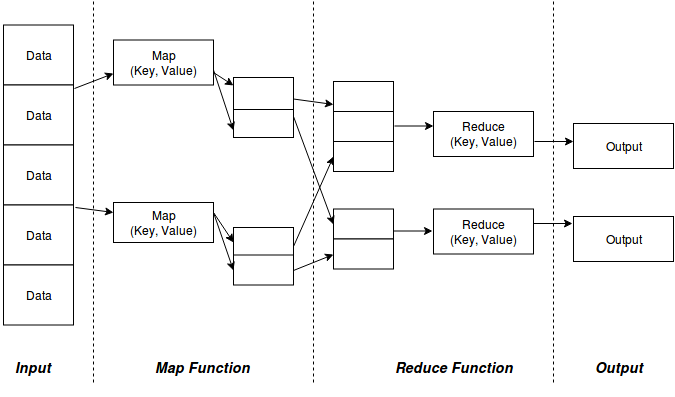
\includegraphics[width =\columnwidth]{Documents/Figures/Mapreduce.png}
    \caption{Figure Data flow in Mapreduce}
    \label{fig:MapreduceDataFlow}
\end{figure}

\noindent Mapreduce eliminates the challenges associated with the traditional approaches to parallel processing of enormous data sets, that is:

\begin{itemize}
    \item Critical path: Time taken to finish the job without delaying the next milestone.
    \item Reliability: A machine fails while working on a data set.
    \item Equal split: Even distribution of data to the machines so as to not overload or under utilize a machine.
    \item Single slip failure: If a machine fails to produce an output. Lack of a failure tolerance capability. 
    \item Agregation of results: Mechanism to collect the results generated by each of the machines to produce the final output
\end{itemize}

\noindent This lab showcases the use of two MapReduce frameworks:  MRJob and Mrs MapReduce. These are python based implementations and were used to perform the lab exercises. MRJob version 0.6.7 was used and Mrs-MapReduce version 0.9 in the lab exercises.
%%%%%%%%%%%%%%%%%%%%%%%%%%%%%%%%%%%%%%%%%%%%%%%%%%%%%%%
\section{Word Count}
\label{sec:WordCount}
\noindent This section looks at a simple word count algorithm of a text. This gives the frequencies of currencies of
words in a text. The algorithms include a lists stop words which are ignored during the word count. The list of Stop Words that were ignored can be seen in Appendix \ref*{app:stopwords}, Table\,\ref{tbl:StopWordsTable}. Both MR Job's and Mrs MapReduce's algorithm follow the pseudo codes provided in Algorithm \ref*{Alg:MapperWordCount} and \ref*{Alg:ReducerWordCount}.

%%%
\begin{figure}[H]
     \removelatexerror
    \begin{algorithm}[H]
       \label{Alg:MapperWordCount}
        \caption{Mapper Algorithm for Word Frequency Count}
        \KwResult{A key and value pair, key equals the word and value is one indicating count}
        \SetKwInOut{Input}{Input}\SetKwInOut{Output}{Output}
        \Input{key}
        \Input{line}
        Split the words in the line text into a list. \\
        Get Stop words list.\\
        \ForEach{word \textbf{in} line}
        {   
            Change word to lowercase.\\
            \If{ word \textbf{not in} STOP\_WORDS \textbf{and} word \textbf{is not} a digit}
            {
                \Return word, 1
            }
        }
    \end{algorithm}
\end{figure}
%%
\begin{figure}[H]
     \removelatexerror
    \begin{algorithm}[H]
       \label{Alg:ReducerWordCount}
        \caption{Reducer Algorithm for Word Frequency Count}
        \KwResult{A key and value pair, key equals the word and value is the total frequency count}
        \SetKwInOut{Input}{Input}\SetKwInOut{Output}{Output}
        \Input{key}
        \Input{frequency list}
        Sum the frequencies.\\
        totalFrquency = sum(frequency)\\
        \Return word, totalFrquency
    \end{algorithm}
\end{figure}

%Consider words to be case-insensitive.
%%
\subsection{MRJob}
%
MRJob implements the word count problem simply by making use of Algorithm\,\ref*{Alg:MapperWordCount}\,and\,\ref*{Alg:ReducerWordCount}. The library reads in the text file and the mapper receives a key which is \emph{None} and a line of text from the text file \cite{ELEN4020A_REF:MRJob067}. The algorithm is run by executing Listing \ref*{lst:MRJobWordCount} in the command line terminal.
%
\begin{center}
\begin{minipage}{0.95\columnwidth}
\begin{lstlisting}[style=bashStyle, label=lst:MRJobWordCount, caption = Command to execute Word Count using MRJob]
python runWordCount.py <filename>
\end{lstlisting}
\end{minipage}
\end{center}
%
The output of the reducer algorithm in the word count script gets printed by the MRJob library to the terminal. The result will simply be the words discovered and their frequency.
%
\subsection{Mrs MapReduce}
Mrs MapReduce has a similar implementation to MRJob. The text file is read and the words are fed to the mapper, then reduced to form a list of words with their frequency of occurrence.
The script is executed using the command in Listing \ref*{lst:MrsWordCount}.
\begin{center}
\begin{minipage}{0.95\columnwidth}
\begin{lstlisting}[style=bashStyle, label=lst:MrsWordCount, caption = Command to execute Word Count (Mrs)]
$ python run_word_count.py <filename>
\end{lstlisting}
\end{minipage}
\end{center}
The output of the program is written to a file in the out put directory given as: \emph{"outPut/source\_0\_split\_0\_.mtxt"}. The output directory is specified in the \emph{run\_word\_count.py} script and it is the same everytime when the program is ran. 
%%%%%%%%%%%%%%%%%%%%%%%%%%%%%%%%%%%%%%%%%%%%%%%%%%%%%
\section{Top K Query}
Top-K query algorithm makes use of the word frequency list produced by the word count algorithm, to give out the top K most frequently occurring words, ignoring stop words. The algorithm does the computations for $K = 10$ and $20$.  Both MR Job's and Mrs MapReduce's algorithms follow the mapper and reducer pseudo codes in Section\,\ref{sec:WordCount} Algorithms\,\ref{Alg:MapperWordCount}\,and\,\ref{Alg:ReducerWordCount}.
%%

%%%
\begin{figure}[H]
     \removelatexerror
    \begin{algorithm}[H]
       \label{Alg:SortingTopKQuery}
        \caption{Sorting Algorithm for Top-K Query}
        \KwResult{A word list sorted in descending order of frequency}
        \SetKwInOut{Input}{Input}\SetKwInOut{Output}{Output}
        \Input{word}
        \Input{frequency}
        Iterate through the list and sort by frequency from highest to lowest.\\
        \Return A sorted list
    \end{algorithm}
\end{figure}
%%%
\begin{figure}[H]
     \removelatexerror
    \begin{algorithm}[H]
       \label{Alg:TruncateTopKQuery}
        \caption{Algorithm to return Top-K Words list}
        \KwResult{A word list with Top-K distinct words}
        \SetKwInOut{Input}{Input}\SetKwInOut{Output}{Output}
        \Input{word}
        \Input{frequency}
        Iterate through the list and print the k elements.\\
        \Return A list of k items of distinct words
    \end{algorithm}
\end{figure}

\subsection{MRJob}
%
For this task, the output of the reducer is saved to a list in memory and it gets sorted in descending order of frequency. Algorithm \ref*{Alg:SortingTopKQuery} is used to achieve the sorting. The sorted list, gets truncated using Algorithm\,\ref*{Alg:TruncateTopKQuery} and the Top K distinct words are printed to the terminal. The script for this task can be executed using the command in Listing\,\ref*{lst:MRJobTopKQuery}.
%
\begin{center}
\begin{minipage}{0.95\columnwidth}
\begin{lstlisting}[style=bashStyle, label=lst:MRJobTopKQuery, caption = Command to execute Top-K Query using MRJob]
python runTopKQuery.py <filename>
\end{lstlisting}
\end{minipage}
\end{center}
%
\subsection{Mrs MapReduce}
%
For Top K Query, the main script runs the word count script first so that the output can be captured. Before the script is ran output directory to make sure that the output is always in the same file. The script will the produce a new output directory and store the results there. The main script will then access the output file, read its content and feed it to a function to sort the list. The sorting of the list is done by Algorithm\;\;\ref*{Alg:SortingTopKQuery}, which sorts them in descending order base on their frequency of occurrence. The list is then truncated using Algorithm\;\;\ref*{Alg:TruncateTopKQuery} to print the top K distinct words. The script is executed using the command in Listing \ref*{lst:MrsTopKQuery}.
%
\begin{center}
\begin{minipage}{0.95\columnwidth}
\begin{lstlisting}[style=bashStyle, label=lst:MrsTopKQuery, caption = Command to execute Top K Query (Mrs)]
$ python runTopKQuery.py <filename>
\end{lstlisting}
\end{minipage}
\end{center}
%

%
%%%%%%%%%%%%%%%%%%%%%%%%%%%%%%%%%%%%%%%%%%%%%%%%%%%%%%
\section{Inverted Indexing}
The algorithm produces an inverted index of the text. This involves listing, for each word, the line numbers
of the text that the words occur. The algorithms only list out about 50 lines of the distinct words as instructed. Both MR Job's and Mrs MapReduce's algorithm follow the pseudo codes provided in Algorithm \ref*{Alg:MapperInvertedIndexing} and \ref*{Alg:ReducerInvertedIndexing}.
%%
%%%%
\begin{figure}[H]
     \removelatexerror
    \begin{algorithm}[H]
       \label{Alg:MapperInvertedIndexing}
        \caption{Mapper Algorithm for Inverted Indexing}
        \KwResult{A key and value pair, key equals the word and value is the line number the word appears in.}
        \SetKwInOut{Input}{Input}\SetKwInOut{Output}{Output}
        \Input{key}
        \Input{Value = Line text}
        Receive the key and value.\\
        \ForEach{word \textbf{in} line}
        {   
            Change word to lowercase.\\
            \If{ word \textbf{not in} STOP\_WORDS \textbf{and} word \textbf{is not} a digit}
            {
                \Return word, lineNumber
            }
        }
        
    \end{algorithm}
\end{figure}
%%%%%
\begin{figure}[H]
     \removelatexerror
    \begin{algorithm}[H]
       \label{Alg:ReducerInvertedIndexing}
        \caption{Reducer Algorithm for Inverted Indexing}
        \KwResult{A key and value pair, key equals the word and value is the line numbers the word appears in.}
        \SetKwInOut{Input}{Input}\SetKwInOut{Output}{Output}
        \Input{key}
        \Input{Line number list}
        Appends all line numbers for a word into one list\\
        \Return word, line number list
    \end{algorithm}
\end{figure}
%%
\subsection{MRJob}
%
The way MRJob reads in a file is different from that in Mrs-MapReduce. The key given as input into the mapper is \emph{None} as stated in the documentation \cite{ELEN4020A_REF:MRJob067}. For the algorithm to work the authors prepended the line numbers to the input file and separated them from the text using a tab character. Algorithm\,\ref*{Alg:MapperMRJobInvertedIndexing} shows the algorithm followed by MRJob's mapper function.
%
\begin{figure}[H]
     \removelatexerror
    \begin{algorithm}[H]
       \label{Alg:MapperMRJobInvertedIndexing}
        \caption{Mapper Algorithm for Inverted Indexing in MRJob}
        \KwResult{A key and value pair, key equals the word and value is the line number it appears in.}
        \SetKwInOut{Input}{Input}\SetKwInOut{Output}{Output}
        \Input{key}
        \Input{Value = Line text}
        Receive the key and value.\\
        In MRJob key is None and value will contain line text with line numbers prepended and separated by a tab.\\
        Split the line text into lineNumber and line at the first tab.\\
        \ForEach{word \textbf{in} line}
        {   
            Change word to lowercase.\\
            \If{ word \textbf{not in} STOP\_WORDS \textbf{and} word \textbf{is not} a digit}
            {
                \Return word, lineNumber
            }
        }
    \end{algorithm}
\end{figure}
%
\noindent For this task, Listing\ref*{lst:MRJobInvertedIndexing} indicates how to execute the code in the command line terminal.
%
\begin{center}
\begin{minipage}{0.99\columnwidth}
\begin{lstlisting}[style=bashStyle, label=lst:MRJobInvertedIndexing, caption = Command to execute Inverted Indexing using MRJob]
python runInvertedIndexing.py <filename>
\end{lstlisting}
\end{minipage}
\end{center}
%
%
%
\subsection{Mrs MapReduce}
%
The Inverted Indexing operates is a similar as the Mrs MapReduce's Top K Query script. The script starts by deleting the output directory if it exists, then instructs the operating system to run the \emph{invertedIndexing.py} script using the filename and the default output directory (named "outPut"). The \emph{invertedIndexing.py} script is a modified word count which reads the distinct words and the list line on which they occur. The main algorithms for mapping the words with the lines and then reducing them  are shown in Algorithm \ref*{Alg:MapperInvertedIndexing} and \ref*{Alg:ReducerInvertedIndexing} respectively. The Inverted Indexing script can be executed by using the command in Listing \ref*{lst:MrsInvertedIndexing}.
%
\begin{center}
\begin{minipage}{0.99\columnwidth}
\begin{lstlisting}[style=bashStyle, label=lst:MrsInvertedIndexing, caption = Command to execute Inverted Indexing (Mrs)]
python runInvertedIndexing.py <filename>
\end{lstlisting}
\end{minipage}
\end{center}
%
%%%%%%%%%%%%%%%%%%%%%%%%%%%%%%%%%%%%%%%%%%%%%%%%%%%%%%%
\section{Analysis of Results}
To analyze the performance of the MapReduce frameworks implemented, the authors ran the python scripts on a desktop computer with the following specs: an Intel Core i7-6700 CPU with 8\,cores running at 3.40\,GHz and 8\,GB DDR3\,RAM and on the Wits EIE Hornet01 Linux computer which has 8\,cores running at 3.40\,GHz and 16\,GB RAM. Both computers were running Ubuntu with the only difference that the desktop was using version 16.04 LTS and the Hornet01 was running Ubuntu 18.04.2 LTS.\\

\noindent The text files generated for testing were \emph{File1ForLab3.txt} which contained only 34 lines of text and \emph{File2ForLab3.txt} which contained 1407 lines of text. 
%
\subsection{MRJob}
%
The MRJob's jobs were tested in local runner configurations for the runners. A local runner runs MRJob in multiple sub-processes for each task \cite{ELEN4020A_REF:MrJobLocalRunner} .\\

\noindent The average time taken to execute the jobs were taken down in seconds and the results can be seen in Appendix \ref*{app:Results} Table\,\ref{tbl:MRJobLocalRunnerResults}.
%%%%%
\noindent The scripts were executed three times and the average of the results were taken down.\\

 \noindent From the results, it an be seen that the local runner configuration performs better on Hornet01 than it does on the Desktop PC for both input files. The speed differences might be because Hornet01 is configured to run workloads in parallel and MRJob would try to run the workloads across the Desktop PC's cores. The variance in results may be due to the configuration of the Hornet01 computer.
%%%%%
\subsection{Mrs MapReduce}
%
Mrs MapReduce was only tested as a local runner. This allowed for the jobs to be split into sub-processes. All the Mrs MapReduce scripts had a runner script because the Mrs' reduce function has an exit script command which closes the script without return to where it was called. The runner script was used to time the main algorithm's performance. The scripts were ran at least five times and the average time in seconds was recorded. The results can be observe in Appendix\;\;\ref*{app:Results} Table\;\;\ref{tbl:MrsMapReduceResults}.

\noindent From the results, it can be seen that scripts took longer to compute on the Desktop PC as compared to when they were ran on Hornet01. This is mainly because Hornet01 is configured to run workloads in parallel.
%
\subsection{MRJob vs Mrs-MapReduce}
When processing \emph{File1ForLab3.txt} on Hornet01, MRJob in Local runner configuration and Mrs-MapReduce have similar execution times. This is not the same when processing the larger text in \emph{File2ForLab3.txt}, where it can be seen that MRJob in Local runner configuration is faster than Mrs-MapReduce by as much as approximately 400\,ms and a minimum of approximately 200\,ms.\\

\noindent On the Desktop PC, MRJob performed better than Mrs-MapReduce on both files in most cases. The differences in processing times might be due to the differences in how the libraries were coded and the fact that one needs to read Mrs-MapReduce's reducer output from a text file. Reading the data from the disk could increase the processing time.

%%%%%%%%%%%%%%%%%%%%%%%%%%%%%%%%%%%%%%%%%%%%%%%%%%%%%%%%%%%%%%
\section{Conclusion}
%
This report detailed the use of MRJob and Mrs-MapReduce, in Python, to solve simple problems using a MapReduce approach. It was observed that MRJob in local runner configuration generally performed better on all tasks than Mrs-MapReduce on both Hornet01 and on the Desktop PC for both large and small texts. Both frameworks provided an easy way to perform MapReduce tasks and are documented well.
%
\bibliographystyle{IEEEtran}
\bibliography{IEEEabrv,ELEN4020A_REF}
%%%%%%%%%%%%%%%%%%%%%%%%%%%%%%%%%%%%%%%%%%%%%%%%%%%%%%%%%%%%%%%%%%%%%%%%%%%%%%%%%%%%%%%%%%%%%%%%%%%%%%%%%%%%%%%%%%%
\cleardoublepage
\onecolumn
\appendix
%%%%%%%%%%%%%%%%%%%%%%%%%%%%%
%%%%%%%%%%%%%%%%%%%%%%%%%%%%%%%%%%%%%%%%%%%%%%%%%%%%%%%%%%%%%%%%%%%%%%%%%%%%%%%%%%%%%%%
\section{Stop Words}
\label{app:stopwords}
%
\begin{table}[H]
\centering
\caption{Table showing a list of stop words used.}
\label{tbl:StopWordsTable}
\begin{tabular}{|c|}
\hline
\textbf{Stop Words}                                                    \\ \hline
\textit{"a","about","above","after","again",}                          \\
\textit{"against", "all", "am", "an", "and", "any", "are",}            \\
\textit{"as", "at", "be", "because", "been", "before", "being",}       \\
\textit{"below", "between", "both", "but", "by", "could", "did",}      \\
\textit{"do", "does", "doing", "down", "during", "each", "few",}       \\
\textit{"for", "from", "further", "had", "has", "have", "having",}     \\
\textit{"he", "he'd", "he'll", "he's", "her", "here", "here's",}       \\
\textit{"hers", "herself", "him", "himself", "his", "how", "how's",}   \\
\textit{"i", "i'd", "i'll", "i'm", "i've", "if", "in", "into", "is",}  \\
\textit{"it", "it's", "its", "itself", "let's", "me", "more", "most",} \\
\textit{"my", "myself", "nor", "of", "on", "once", "only", "or",}      \\
\textit{"other", "ought", "our", "ours", "ourselves", "out", "over",}  \\
\textit{"own", "same", "she", "she'd", "she'll", "she's", "should",}   \\
\textit{"so", "some", "such", "than", "that", "that's", "the",}        \\
\textit{"their", "theirs", "them", "themselves", "then", "there",}     \\
\textit{"there's", "these", "they", "they'd", "they'll", "they're",}   \\
\textit{"they've", "this", "those", "through", "to", "too", "under",}  \\
\textit{"until", "up", "very", "was", "we", "we'd", "we'll", "we're",} \\
\textit{"we've", "were", "what", "what's", "when", "when's", "where",} \\
\textit{"where's", "which", "while", "who", "who's", "whom", "why",}   \\
\textit{"why's", "with", "would", "you", "you'd", "you'll", "you're",} \\
\textit{"you've", "your", "yours", "yourself", "yourselves"}           \\ \hline
\end{tabular}
\end{table}

\section{Results}
\label{app:Results}
\subsection{MRJob}
%%%%%
\begin{table}[H]
\centering
\caption{Table showing time taken in seconds to execute MRJob with a local runner}
\label{tbl:MRJobLocalRunnerResults}
\begin{tabular}{|l|l|l|l|l|l|l|}
\hline
\multicolumn{7}{|c|}{\textbf{MRJob's Runner in Local Mode}}                                                                                                                                                 \\ \hline
\textbf{}                         & \multicolumn{2}{c|}{\textbf{Word Count}}                                  & \multicolumn{2}{c|}{\textbf{Top K Query}} & \multicolumn{2}{c|}{\textbf{Inverted Indexing}} \\ \hline
 &\multicolumn{1}{l|}{\textbf{PC}} & \multicolumn{1}{l|}{\textbf{Hornet01}} & \textbf{PC}      & \textbf{Hornet01}      & \textbf{PC}         & \textbf{Hornet01}         \\ \cline{1-7} 
File1ForLab3.txt                                  & 0.349227458                      & 0.145003454                            & 0.292195913      & 0.151581794            & 0.292010370         & 0.129592853               \\ \hline
File2ForLab3.txt                  & 0.447210146                      & 0.309454827                            & 0.397815861      & 0.267846315            & 0.414259918         & 0.354714417               \\ \hline
\end{tabular}
\end{table}
%%%%%
\subsection{Mrs MapReduce}
\label{app:MrsResults}
%
\begin{table}[H]
\centering
\caption{Table showing time taken in seconds to execute Mrs Map Reduce.}
\label{tbl:MrsMapReduceResults}
\begin{tabular}{|l|l|l|l|l|l|l|}
\hline
\multicolumn{7}{|c|}{\textbf{Mrs Map Reduce}}                                                                                                                                                               \\ \hline
\multicolumn{1}{|c|}{\textbf{}}   & \multicolumn{2}{c|}{\textbf{Word Count}}                                  & \multicolumn{2}{c|}{\textbf{Top K Query}} & \multicolumn{2}{c|}{\textbf{Inverted Indexing}} \\ \hline
 & \multicolumn{1}{c|}{\textbf{PC}} & \multicolumn{1}{c|}{\textbf{Hornet01}} & \textbf{PC}      & \textbf{Hornet01}      & \textbf{PC}         & \textbf{Hornet01}         \\ \cline{1-7} 
File1ForLab3.txt                                  & 0.334859609                      & 0.157367229                            & 0.363074302      & 0.159703254            & 0.415356397         & 0.157572984               \\ \hline
File2ForLab3.txt                  & 1.233693599                      & 1.230403423                            & 1.351403713      & 1.410311222            & 1.896836280         & 1.556517839               \\ \hline
\end{tabular}
\end{table} 
\end{document}